%Chapter 2: Seismogeodesy and Strong Motion Sensing

\chapter{Seismogeodesy and Strong Motion Sensing}

\section{Strong Motion Seismology}
The range of motions produced by the seismic source is broad both in frequency and dynamic range. It is well known that no one sensor can capture all signals of interest to seismology and earthquake engineering \citep{Havskov2006}. Seismologists typically rely on seismometers, whose response is related to velocity of the ground, for measurement of small amplitude signals (weak motion), but for large amplitude signals these sensitive instruments saturate or clip. In this case, strong motion sensors, whose response is related to the acceleration of the ground and have lower gains, are preferred. Modern observatory grade accelerometers rely on the force feedback principle and can measure motions as small as 1 nm at 1 Hz and 100 nm at 0.1 Hz and accelerations of up to 4g. Furthermore their frequency response is flat from ) (often called the DC-level) to 50-200 Hz \citep{Havskov2006}.

Thus, in principle there should be no difficulty in integrating a strong motion record to velocity and displacement. This is not the case; in practice the simple integration of an accelerogram produces unphysical velocity and displacement waveforms that grow unbounded as time progresses. Computation of broadband displacements from strong motion recordings is a thoroughly studied procedure that is fraught with many known problems and has no known single solution. By ``broadband dispalcement'' it is meant a strong motion displacement waveform that captures both transient phenomena (waves) and permanent or static deformation, i.e. a recording reliable from DC to the Nyquist frequency.

The problems associated with the double integration of accelerometer recordings have been comprehensively studied and many sources of error have been suggested: numerical error in the integration procedure, mechanical hysteresis, cross-axis sensitivity and unresolved rotational motions \citep{Graizer1979,Iwan1985,Boore1999,Boore2001,Boore2002,Smyth2007}. It is generally assumed that small offsets are introduced in the acceleration time series; upon integration these baseline offsets produce the linear and quadratic trends observed in the velocity and displacement time series, respectively. Many possible sources have been invoked as the source of these offsets with unresolved rotational motion increasingly considered the main error \citep{Graizer2006,Pillet2007}. Motion is described by six degrees of freedom, three translations and three rotations. Accelerometers are incapable of discerning between rotational and translational motions, thus, rotational motions are recorded as spurious translations. Effectively, this results in a change of the baseline of the accelerometer, even if by a small amount, leading to unphysical drifts in the singly integrated velocity waveforms and doubly integrated displacement waveforms (Figure \ref{fig_iwt009}).

\begin{figure}[!ht] 
  \centering
  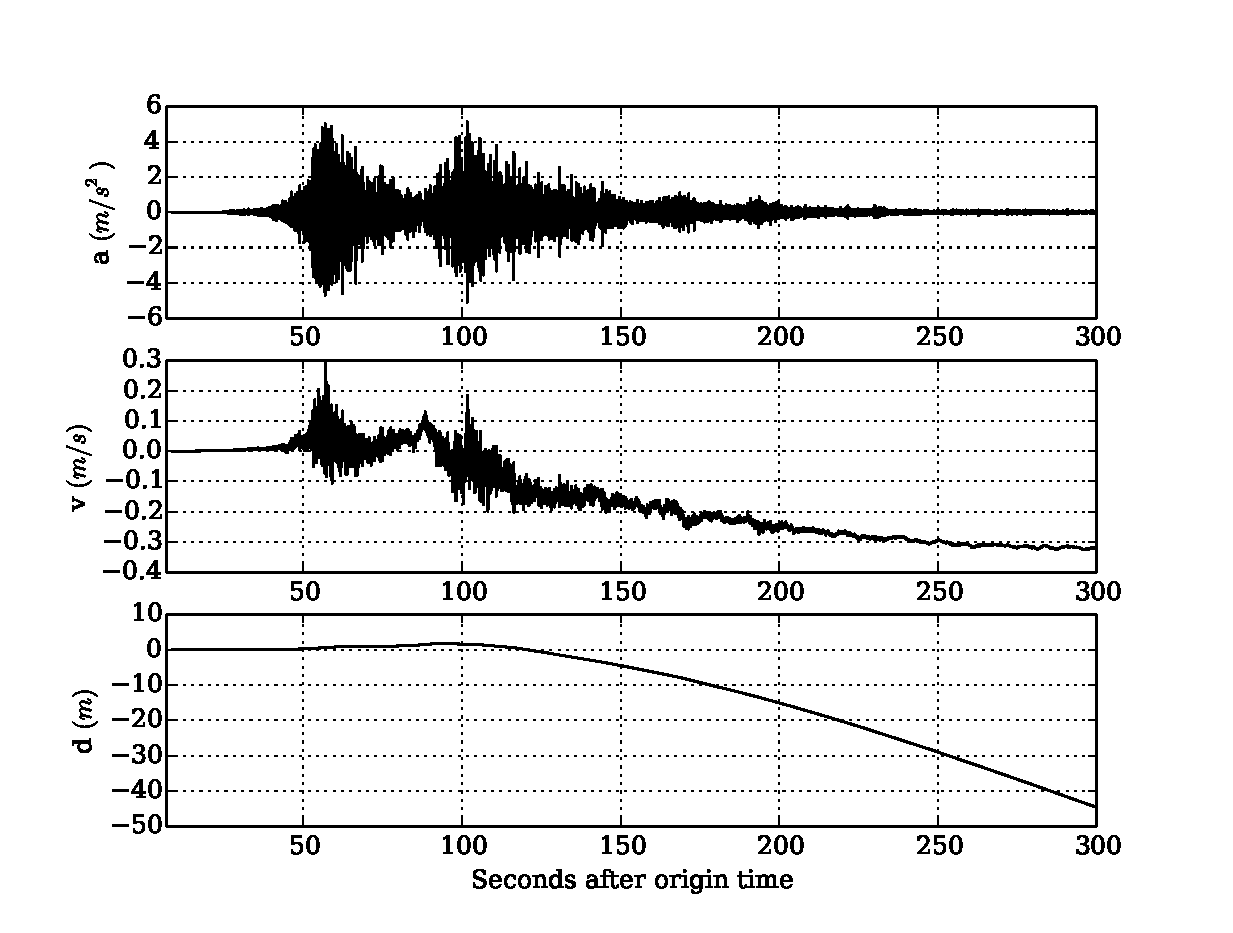
\includegraphics[width=0.99\linewidth]{./figures/iwt009.eps}
    \caption[Effect of numerical integration on a strong motion recording.]{Effect of numerical integration on a strong motion accelerogram. This example is for the east component of motion at station IWT009 192 km from the centroid of the 2011 M9 Tohoku-oki earthquake. Note the unphysical drifts in both the velocity and displacement time series.}
  \label{fig_iwt009}
\end{figure}

Many correction schemes, collectively known as baseline corrections, have been proposed over time to deal with this problem. Rotational motions become more prevalent close to the source and at long periods. In particular \citet{Trifunac2001} have shown that rotational motions have significant contributions to radiated spectra and can sometimes be the predominant source of seismic energy, particularly at very long periods and for very large earthquakes. 

The simplest baseline correction scheme is a high-pass filter \citep{Boore2005}. This leads to accurate recovery of the mid to high frequency part of the displacement record but suppresses completely long period information such as the static offset (Figure \ref{fig_iwt009bl}). To ameliorate this, a number of more elaborate correction schemes exist \citep{Boore2005} that rely on function fitting to the singly integrated velocity time series. The most reliable scheme that routinely produces plausible displacement waveforms (which include a measure of the static offset) is described in \citet{Boore1999, Boore2001} and is a modification of the scheme proposed by \citet{Iwan1985} and henceforth referred to as the Boore-Iwan or BI correction scheme. In this method a piece-wise linear function is fit to the uncorrected velocity time series, the slope of each straight line segment represents an acceleration step which is then subtracted from the original acceleration data. This baseline corrected acceleration record is subsequently integrated to velocity and displacement. If the intervals for fitting the linear functions to the velocity data are selected appropriately this algorithm will produce waveforms that look plausible. They will contain both permanent and transient motions. The difficulty then lies in determining what these appropriate time intervals are from the data themselves. As discussed by \citet{Boore1999,Boore2001} this is an ambiguous process. To diminish this uncertainty, subsequent research has focused on determining plausible times for the fits and then grid searching for waveforms that most resembles a ramp or step function \citep{Wu2007,Chao2010,Wang2011}.

This is better understood through an example. Consider the time series of Figure \ref{fig_iwt009}. The traditional BI correction procedure starts by removing the pre-event mean or baseline, this is called the zeroth order corrected waveform. Then for some analyst determined initial correction time time $t_i$ and final correction time $t_f$, two baselines or acceleration steps can be computed from the drift in the velocity data and subsequently removed. Underlying this process is the assumption that from time $t_i$ to some intermediate time $t_1$ (determined by the analyst) a baseline offset due to strong shaking is introduced into the time series and subsequently from this intermediate time $t_1$ to the final correction time $t_f$ a \textit{permanent} baseline offset is introduced into the data. Thus, the first acceleration step is determined by a least squares straight line fit to the velocity data between times $t_1$ and $t_f$ such that
\begin{equation}
v_f(t)=v_0+a_f(t)\;;\;t\in(t_1,t_f)\;,
\end{equation}
where the regression parameters are $v_0$ and the acceleration step $a_f$. Subsequently, another straight line is fit from $t_i$ to $t_1$ with the constraint that velocity be zero at the start of the record and that the final velocity averages to zero. These constraints are satisfied if \citep{Boore1999}
\begin{equation}
am=\frac{v_f(t_1)}{t_1-t_i}\;.
\end{equation}
Then, the acceleration baseline, $a_m$, is subtracted from the uncorrected record from times $t_i$ to $t_1$ and the baseline offset, $a_f$, is subtracted from the zeroth order corrected record for times $t_1$ to $t_f$. The record is then integrated to velocity and displacement. This scheme produces waveforms that look plausible; they contain both transient and permanent motions. However an ambiguity lies in the selection of times $t_i$ and $t_1$. As has been amply discussed by \citet{Boore1999,Boore2001}, this ambiguity is not easily resolved without external information and each investigator relies on subjective judgment to ascertain what looks best. Figure \ref{fig_iwt009bl} illustrates such an example where the same waveform has been baseline corrected for several values of $t_1$ while holding $t_i$ fixed at the P wave arrival time with results that vary wildly. If the waveform is complex, as in this example, which has two distinct pulses of very strong shaking, then more baselines might need to be subtracted. However, if there is already ample ambiguity in the simple determination of the two baselines $a_m$ and $a_f$, the problem is exacerbated with the introduction of more baselines. 

\begin{figure}[!ht] 
  \centering
  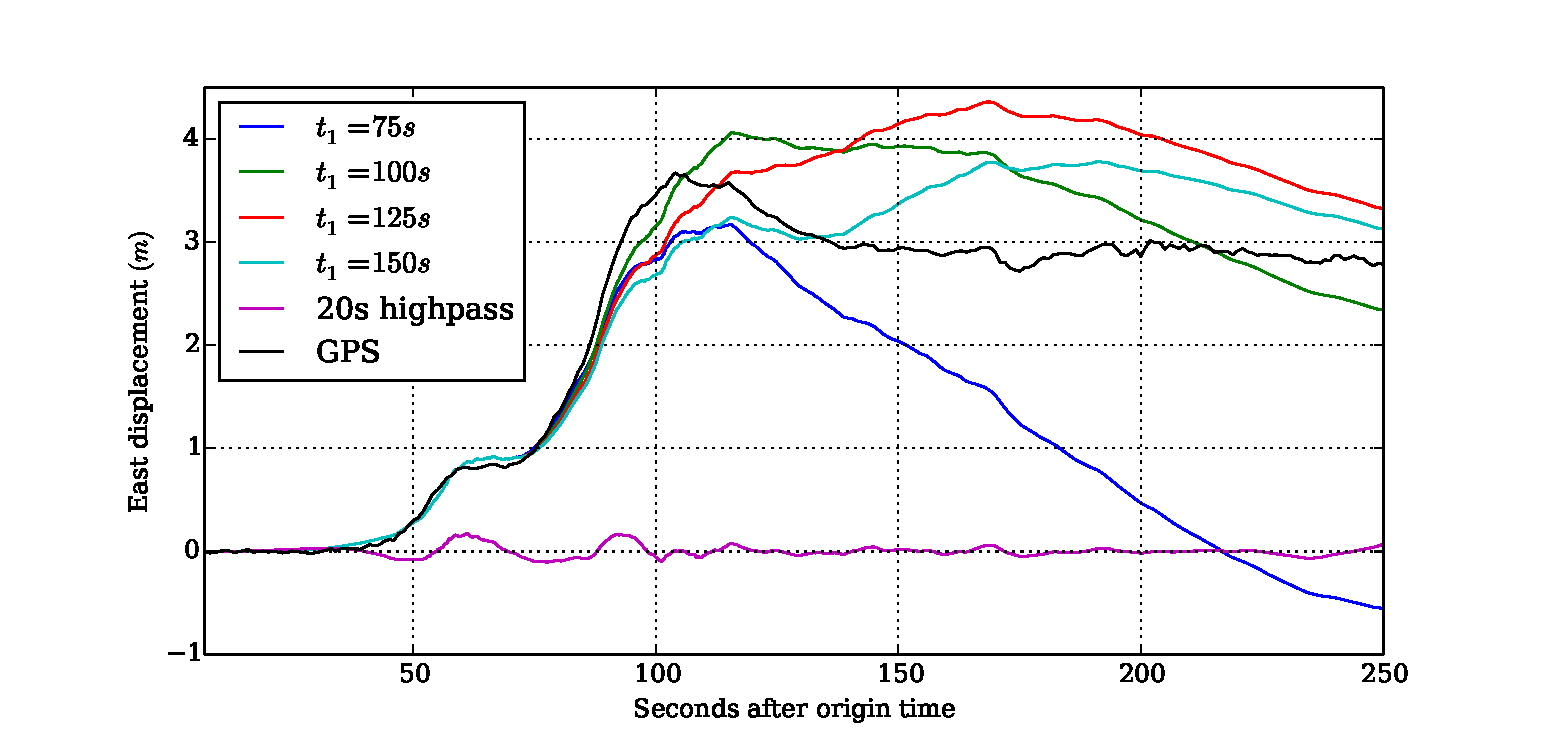
\includegraphics[width=0.99\linewidth]{./figures/iwt009bl.eps}
    \caption[Some simple baseline corrections.]{Baseline corrections using the BI algorithm for the east component of motion at station IWT009 192 km from the centroid of the 2011 M9 Tohoku-oki earthquake using different values of the correction parameter $t_1$. Also shown is the result of a 20s high pass filter corrected waveform and the GPS displacements recorded at the same site}
  \label{fig_iwt009bl}
\end{figure}

The correction times $t_i$ and $t_1$ can and do vary for each station-event pair and even for different channels at the same station during the same event. Practically this means that analysis of broadband displacements from baseline-corrected accelerometer records is inherently ambiguous and complicated for real-time seismological applications or across large networks both for real-time and post-processing purposes.

Research into automated baseline correction from accelerometer data alone has focused on variations of the BI scheme. \citet{Wu2007} proposed a variant in which the times for each linear segment of the baseline correction are determined by a grid search such that the resulting time series best matches a ramp function. \citet{Chao2010} elaborated on the formulation of \citet{2007} by adding an extra restriction that the times be selected after certain threshold values of acceleration energy have been accrued. Both studies compare their results to static offsets determined from GPS and find that their estimates are somewhat similar. They still maintain some significant differences though, and no analysis on the adequacy of the remaining part of the waveform is performed. It is implicitly assumed that if the static field is well fit then the rest of the waveform will be reliable as well.

An important advance in automatic baseline correction is presented in \citet{Wang2011} who present another variation of the BI bilinear scheme that performs better than those discussed thus far. They develop some simple rules for determination of the interval of possible correction times based on analysis of the uncorrected acceleration and displacement waveforms. From an analysis of the time at which the peak ground acceleration (PGA) occurs and the time of last zero crossing in the uncorrected displacement they determine bounds for the grid search of baseline correction times. They then perform the grid search among these possible correction times and fit, via a non-linear regression, a step function to all possible waveforms. An optimum correction (the one that best fits this step function) is then selected. Unlike previous studies they compare their results not only to measured static offsets but to observed 1 Hz GPS data; they do this for a single station. They find for that one station an error of \~20\% in the static field estimation but a very good agreement between the corrected displacement and the GPS for the first 200s of the waveform.

In a follow up study \citet{Wang2013} apply their methodology to accelerometer records for the 2011 Mw 9.0 Tohoku-oki earthquake. They obtain reasonable estimates of the static field for many stations in the KiK-net network in Japan but also find numerous outliers. They then develop a simplified scheme to screen the outliers by excluding coseismic offsets that deviate more than 15° from the predictions of a static slip inversion. Furthermore, they compare their automatic corrections for selected borehole sensors in the KiK-net network with nearby high-rate GPS stations with mixed results. They find that while parts of the waveforms might be a good match, the static estimates can be in error by a significant amount. To ameliorate this they then propose to use the static field from nearby GPS stations as a constraint in the correction procedure. From the pool of all candidate baseline corrections they select the one that fits a step function of amplitude given by the static field. It is noteworthy that \citet{Wang2013} do not provide baseline corrected solutions for the sister strong motion network K-net. They readily acknowledge that K-net stations, which generally have less favorable site responses \citep{Tsuda2006}, are not well modeled by this automatic approach. 

%Network correction

\section{The role of GPS}

An alternative to baseline corrections of strong motion data is to measure displacements directly using the  Global Positioning System (GPS). There are two basic approaches to precise GPS data analysis: network positioning and precise point positioning. In both approaches stations positions are estimated with respect to a global Cartesian terrestrial reference system. This system is realized by the published coordinates and velocities of hundreds of global geodetic stations in the International Terrestrial Reference Frame (ITRF). Precise GPS satellite orbital products distributed by the International GNSS Service (IGS) are tied to this underlying reference frame, and without loss of generality, are assumed to be fixed in the GPS data analysis. 

In network positioning, data from a network of stations are analyzed simultaneously to estimate station positions and integer-cycle phase ambiguities \citep{Dong1989,Blewitt1989}, and other parameters such as zenith troposphere delays. Analyzing the data as a network, results in the effective cancellation of GPS receiver clock and satellite clock errors, which are common to multiple satellite and stations, respectively. Precise point positioning \citep{Zumberge1997} relies on fixed satellite orbits, as well as satellite clock parameters also available through the IGS and/or its different analysis centers . These parameters are held fixed in the process of estimating ITRF positions of individual CGPS stations, phase ambiguities, zenith troposphere delays and station clock parameters.

Network positioning and precise point positioning approaches can be considered equivalent, in terms of the underlying physics. However, to achieve geodetic quality positions (mm- to cm-level), it is essential to resolve integer-cycle phase ambiguities to their correct integer values \citep{Blewitt1989,Dong1989}. This is straightforward for batch post-processing, which includes the simultaneous analysis of multiple GPS data records, usually sampled at rates of 15-30 s, to derive a single station position over the entire sampled interval. It is the source of the typical 24-hour GPS position time series used to study permanent deformation, including long-term tectonic motion, as well as coseismic, postseismic and other transient deformation. Batch post-processing plays a role in seismological applications by providing highly-accurate, true-of-date ITRF station positions with respect to which displacement waveforms can be estimated during an event. There are several analysis groups that are producing 24-hour position time series on an operational basis.

%here
Of primary importance in seismological applications is the estimation of cm-level or better displacements at the GPS receiver sampling rate, typically 1 Hz. Since the first pioneering efforts over a decade ago \citep{Nikolaidis2001,Larson2003,Bock2004,Miyazaki2004} post-processed single-epoch network positioning with resolution of integer-cycle phase ambiguities is now routinely applied to seismology.  However, a general real-time solution is still elusive, and analysis of multiple data epochs is usually required to resolve integer-cycle phase ambiguities and estimate single-epoch positions.
Precise point positioning has been limited in GPS seismology, in particular for real-time applications, because of unresolved integer-cycle phase ambiguities and slow convergence rates and re-convergence rates when loss of lock on the satellite signals occurs. JPL’s Global Differential GPS (GDGPS) System employs a large global ground network of real-time reference receivers and real-time data processing software, which allows a single GPS receiver to be point positioned with 10-20 cm accuracy anywhere in the world. This level of accuracy is considered useful for global tsunami warning generated by great earthquakes (Bar-Sever et al., 2009). A relatively new area of geodetic research is rapid integer cycle ambiguity resolution in precise point positioning, without the need for specific reference stations. Besides fixed satellite orbits and clocks, and estimation of positions, receiver clocks and tropospheric delays of the GPS signals, it also requires prediction of ionospheric delays. Recent results have been encouraging in that reliable ambiguity resolution and cm-level positioning accuracies have been achieved with only a few epochs of 1 Hz GPS data for re-convergence, although about a 20 minute convergence period is still required (e.g., Geng 2010).




The availability of suitably correction algorithms for strong motion waveforms that can produce broadband displacements is of broad interest, especially for source analysis and hazards assesment.. Indeed there is ample interest in access to such real-time broadband displacements. Static offsets have been used for rapid source dimension computations [Perez-Campos et al. 2013; Crowell et al. 2013] and centroid moment tensor (CMT) determination of large sources [Melgar et al. 2012; Crowell et al., 2013]. It has been demonstrated as well that such algorithms can provide rapid descriptions of the source in a timelier and complete manner than traditional seismic data. Static slip inversions can also be computed rapidly with such data [Crowell et al. 2012, 2013; Wright et al., 2012] and ingested into rapid models of the ensuing tsunami [Ohta et al., 2012]. Except for select locales like the U.S. and Japan, Global Positioning System (GPS) networks with enough density to adequately capture large events are not as prevalent as strong motion deployments, thus extracting reliable long period information that includes the static field, from accelerometer data alone, would be very valuable. Furthermore, inversions with regional high-rate GPS data that model both the static and dynamic components of the waveform have been demonstrated for CMT determination [O’Toole et al., 2012, 2013] and kinematic slip inversions [Ji et al., 2004; Ammon et al., 2011]. However, the low sampling rates of GPS (~1-5 Hz) and its high noise levels compared to seismic data make full waveform inversions from GPS data alone suspect. Hence such inversions are usually leveraged with teleseismic data. This is unsuitable for rapid analysis of sources at regional scales and it makes access to broadband displacements, as would ostensibly be produced from baseline corrections, very appealing.

%\appendix
%\chapter{Final notes}
%  Remove me in case of abdominal pain.

